\documentclass{../../slides-style}

\slidetitle[Требования, рекомендации]{Учебные практики второго курса}{28.09.2024}

\begin{document}

    \begin{frame}[plain]
        \titlepage
    \end{frame}

    \begin{frame}
        \frametitle{Что такое учебная практика}
        \begin{itemize}
            \item Научно-исследовательская или программно-инженерная работа%
            \begin{itemize}
                \item Решение более-менее сложной практической либо научной задачи
                \item Отчёт (текст)
                \item Код (опционально, но желательно)
            \end{itemize}
            \item По формату близка к научной статье и выступлению на конференции
            \item Тема должна быть интересна кафедре системного программирования
            \begin{itemize}
                \item Средства разработки, операционные системы, библиотеки и т.п.
            \end{itemize}
        \end{itemize}
    \end{frame}

    \begin{frame}
        \frametitle{Требования}
        \begin{itemize}
            \item Отчёт
            \begin{itemize}
                \item Порядка 5-7 содержательных страниц
            \end{itemize}
            \item Отзыв научного руководителя
            \begin{itemize}
                \item С подписью, к дате зачёта
            \end{itemize}
        \end{itemize}
    \end{frame}

    \begin{frame}
        \frametitle{Кто такой научник, консультант и т.п.}
        \begin{itemize}
            \item \textit{Консультант} --- ставит задачу, читает и рецензирует код, помогает с техническими проблемами
            \item \textit{Научный руководитель} --- преподаватель (обязательно), отвечает за адекватность задачи, следит за методологическими вопросами, следит за ходом работы, помогает с текстом и подготовкой к защите
            \item \textit{Руководитель практики} --- общая организация процесса, сбор и распределение тем, сбор отчётов и отзывов, организация защит, решение организационных проблем
            \item \textit{Комиссия} --- преподаватели кафедры, представитель индустрии
            \begin{itemize}
                \item Все защиты всегда с комиссией
            \end{itemize}
        \end{itemize}
    \end{frame}

    \begin{frame}
        \frametitle{Откуда брать тему и научного руководителя}
        \begin{itemize}
            \item Сайт кафедры: \url{https://se.math.spbu.ru/diplomas/index.html}
            \begin{itemize}
                \item Обратите внимание, там есть фильтры
                \item Если тема заинтересовала, но не подходит, можно пообщаться с консультантом
            \end{itemize}
            \item У преподавателя по программированию --- он сможет хотя бы направить
            \item На стажировке
            \item Если были в ЛШ --- продолжить начатое
            \item Определиться с выбором темы надо \textbf{за первую неделю октября}
        \end{itemize}
    \end{frame}

    \begin{frame}
        \frametitle{Примерный план работы}
        \begin{itemize}
            \item Сентябрь --- определиться с научным руководителем и темой
            \item Сентябрь-начало декабря --- работа над практикой
            \begin{itemize}
                \item Быстрый мини-обзор
                \item Введение, постановка задачи, научиться убеждать окружающих в актуальности темы
                \item Обзор
                \item Проектирование
                \item Реализация (если предполагалась)
                \item Апробация/эксперименты (если предполагались)
                \item Написание текста
            \end{itemize}
            \item Конец декабря --- защиты
        \end{itemize}
    \end{frame}

    \begin{frame}
        \frametitle{Сроки}
        \begin{itemize}
            \item Работа может писаться семестр, год, два и т.д., но отчётность каждый семестр
            \begin{itemize}
                \item Хотя бы один семестр из двух --- с реализацией
            \end{itemize}
            \item Минимум раз в неделю отчитываться научному руководителю о ходе работы
            \begin{itemize}
                \item Используйте \url{https://se.math.spbu.ru/practice}
            \end{itemize}
        \end{itemize}
    \end{frame}

    \begin{frame}
        \frametitle{Полезные ресурсы}
        \begin{itemize}
            \item Сайт кафедры СП --- \url{https://se.math.spbu.ru/}, там раздел \enquote{Студентам} --- примеры работ
            \item Шаблон отчёта: \url{https://github.com/spbu-se/matmex-diploma-template}
            \item Шаблон презентации: \url{https://github.com/spbu-se/report_presentation_template}
            \item Онлайн-редакторы TeX --- \url{https://papeeria.com/}, \url{https://www.overleaf.com/}
            \item Чеклист по оформлению репозитория: \url{https://github.com/yurii-litvinov/courses/blob/master/additional/repo-checklist/repo-checklist.pdf}
            \item Чеклист по презентации: \url{https://goo.gl/UeDRff}
            \item Все новости, объявления и созвоны --- в команде курса в Teams
        \end{itemize}
    \end{frame}

    \begin{frame}
        \frametitle{Отчёт, структура}
        \begin{itemize}
            \item Титульный лист
            \item Оглавление
            \item Введение в предметную область, постановка задачи
            \item Обзор литературы и существующих решений
            \item Описание предлагаемого решения (архитектура, реализация)
            \item Апробация/эксперименты
            \item Заключение
            \item Список литературы
        \end{itemize}
    \end{frame}

    \begin{frame}
        \frametitle{Введение}
        \begin{columns}
            \begin{column}{0.6\textwidth}
                \begin{itemize}
                    \item Известная информация, \foreignquote{english}{Background}
                    \item Неизвестная информация, \foreignquote{english}{Gap}
                    \begin{itemize}
                        \item Актуальность темы
                        \item Практическая значимость
                        \item Кому конкретно это надо
                    \end{itemize}
                    \item Кратко про ваш подход к решению задачи, почему он приведёт к успеху (\enquote{Гипотеза} и \enquote{Подход})
                \end{itemize}
            \end{column}
            \begin{column}{0.4\textwidth}
                \begin{center}
                    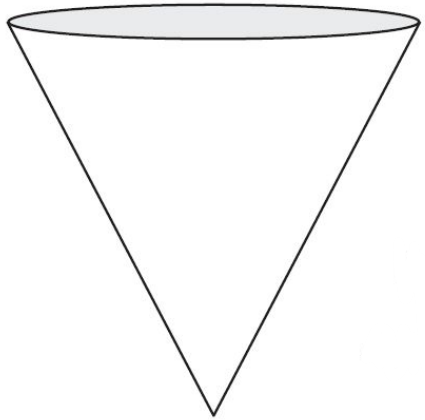
\includegraphics[width=\textwidth]{introductionCone.png}
                \end{center}
            \end{column}
        \end{columns}
    \end{frame}

    \begin{frame}
        \frametitle{Постановка задачи}
        \begin{itemize}
            \item Цель работы
            \begin{itemize}
                \item Одним предложением --- что конкретно надо сделать
            \end{itemize}
            \item Задачи
            \begin{itemize}
                \item Отчуждаемые
                \item Специфичные
                \item Решение которых приведёт к цели
                \item Выполнить обзор, спроектировать, реализовать, выполнить апробацию/эксперименты
            \end{itemize}
        \end{itemize}
    \end{frame}

    \begin{frame}
        \frametitle{Обзор}
        \begin{itemize}
            \item Обзор существующих решений
            \begin{itemize}
                \item Цель обзора, критерии отбора материалов
                \item Критерии сравнения
                \item Таблица с результатами
                \item Выводы
            \end{itemize}
            \item Обзор используемых чужих результатов
            \begin{itemize}
                \item Всё, написанное и придуманное не вами --- в обзор
            \end{itemize}
            \item Должен соотноситься с темой работы
        \end{itemize}
    \end{frame}

    \begin{frame}
        \frametitle{Описание решения}
        \begin{itemize}
            \item Желательно, чтобы разделы соответствовали списку задач
            \item Аргументированное обоснование принятых решений и отказа от альтернатив
            \item Выбор инструментария
            \item Описание архитектуры, алгоритмов и т.п.
        \end{itemize}
    \end{frame}

    \begin{frame}
        \frametitle{Описание решения (2)}
        \begin{itemize}
            \item Рисунки и диаграммы
            \begin{itemize}
                \item Лучше использовать UML --- он стандартный
                \item Подписи
                \begin{itemize}
                    \item Чужие рисунки --- со ссылкой на источник
                \end{itemize}
                \item Ссылки из текста
                \item Сквозная нумерация
            \end{itemize}
            \item Таблицы
            \begin{itemize}
                \item Чтобы было всё видно даже в напечатанном варианте
            \end{itemize}
        \end{itemize}
    \end{frame}

    \begin{frame}
        \frametitle{Апробация}
        \framesubtitle{Или эксперименты}
        \begin{itemize}
            \item Доказать, почему всё, что вы делали, вообще осмысленно
            \item Апробация --- внешняя \enquote{оценка} работы
            \begin{itemize}
                \item Отзывы пользователей, лучше количественные
                \begin{itemize}
                    \item Например, \url{https://www.usability.gov/how-to-and-tools/methods/system-usability-scale.html}
                \end{itemize}
                \item Внедрение, релиз, оценки
                \item Выступления на конференциях
            \end{itemize}
            \item Эксперименты --- численное доказательство, что ваш результат лучше аналогов
            \begin{itemize}
                \item Замеры производительности, точности и т.д.
                \item Отдельная большая наука, не делайте на отвяжись!
            \end{itemize}
            \item Если до апробации не дошли --- опишите продуманный план апробации или экспериментов
        \end{itemize}
    \end{frame}

    \begin{frame}
        \frametitle{Заключение}
        \begin{itemize}
            \item Перечисление результатов, выносимых на защиту
            \item Должно быть согласовано с постановкой задачи (вплоть до полного её повторения)
            \item Должно быть согласовано с текстом
            \begin{itemize}
                \item Никаких результатов из ниоткуда
            \end{itemize}
            \item Если практика предполагает продолжение, реалистичные планы на дальнейшую работу
            \item Обязательно ссылка на репозиторий
            \item Примерно полстраницы
        \end{itemize}
    \end{frame}

    \begin{frame}
        \frametitle{Литература}
        \begin{itemize}
            \item Cсылок примерно как страниц в работе
            \item Обязательно на каждый пункт ссылаться из текста
            \item Лучше ссылаться на научные статьи
            \begin{itemize}
                \item Ещё лучше --- на книги, но по предметной области
                \item Смотрите на индекс Хирша и число цитирований
            \end{itemize}
            \item Реально прочитанные работы
            \begin{itemize}
                \item Всё-таки прочитать бывает полезно
            \end{itemize}
        \end{itemize}
    \end{frame}

    \begin{frame}
        \frametitle{Литература (2)}
        \begin{itemize}
            \item ГОСТ Р 7.0.5-2008
            \begin{itemize}
                \item А.Н. Терехов, Т.А. Брыксин, Ю.В. Литвинов и др., Архитектура среды визуального моделирования QReal. // Системное программирование. Вып. 4. СПб.: Изд-во СПбГУ. 2009, С. 171-196
                \item Порядок --- алфавитный (по авторам), в порядке упоминания в тексте, в хронологическом порядке (если это важно)
                \item Ссылки в тексте --- номер в квадратных скобках: ``блаблабла [1]'' (с пробелом)
            \end{itemize}
            \item В литературу --- только, гм, литературу
            \begin{itemize}
                \item Подстраничные сноски для ссылок на сайты, статьи на Хабре и т.д.
                \item Электронные источники в списке литературы допустимы (надо указывать дату обращения)
            \end{itemize}
        \end{itemize}
    \end{frame}

    \begin{frame}
        \frametitle{Презентация, структура}
        \begin{itemize}
            \item Титульный слайд
            \item Введение (примерно 1-2 слайда)
            \item Постановка задачи (1 слайд)
            \item Обзор (примерно 1 слайд)
            \item Предлагаемое решение (примерно 1 слайд)
            \item Результаты, выносимые на защиту (1 слайд) --- обязательно, последним слайдом
        \end{itemize}
    \end{frame}

    \begin{frame}
        \frametitle{Общие рекомендации}
        \begin{itemize}
            \item Никакого заимствования 
            \begin{itemize}
                \item Сдача чужой работы --- отчисление без права восстановления сразу
                \item Копипаст даже одного предложения без указания источника --- незачёт
                \item Правильно оформленный копипаст --- попросят убрать
            \end{itemize}
            \item Обязательно показать и текст, и презентацию научнику
            \begin{itemize}
                \item Стоит порепетировать выступление
            \end{itemize}
            \item Из презентации должно быть предельно понятно, что и зачем вы делаете (актуальность, сложность работы) и при чём тут СП
            \begin{itemize}
                \item Это один из основных пунктов дискуссии
            \end{itemize}
            \item Озаботьтесь получением отзывов заранее
            \item Код --- CI, юнит-тесты, README, лицензия
        \end{itemize}
    \end{frame}

    \begin{frame}
        \frametitle{FAQ}
        \begin{itemize}
            \item Можно ли писать групповую практику?
            \begin{itemize}
                \item Да, но отчёт и презентация у каждого свои
            \end{itemize}
            \item Засчитывают ли выступление на семинаре/конференции за защиту?
            \begin{itemize}
                \item Нет
            \end{itemize}
            \item Можно ли менять тему и научника?
            \begin{itemize}
                \item Да, но предупредить руководителя практики
            \end{itemize}
            \item Можно ли перезачесть работу, написанную в прошлом году?
            \begin{itemize}
                \item Да, но предупредить руководителя практики
            \end{itemize}
            \item Если научник/консультант/лаборатория/родственник ставит мне зачёт, как его получить в зачётку?
            \begin{itemize}
                \item Никак, учебные практики принимаются комиссией в рамках процедуры независимой оценки качества образования
            \end{itemize}
        \end{itemize}
    \end{frame}

\end{document}